%%%%%%%%%%%%%%%%%%%%%%%%%%%%%%%%%%%%%%%%%%%%%%%%
%% Intro to LaTeX and Template for Homework Assignments
%% Quantitative Methods in Political Science
%% University of Mannheim
%% Fall 2019
%%%%%%%%%%%%%%%%%%%%%%%%%%%%%%%%%%%%%%%%%%%%%%%%

% created by Marcel Neunhoeffer & Sebastian Sternberg


% This template and tutorial will help you to write up your homework. It will also help you to use Latex for other assignments than this course's homework.

%%%%%%%%%%%%%%%%%%%%%%%%%%%%%%%%%%%%%%%%%%%%%%%%
% Before we get started
%%%%%%%%%%%%%%%%%%%%%%%%%%%%%%%%%%%%%%%%%%%%%%%%

% Make an account on overleaf.com and get started. No need to install anything.

%%%%%%%%%%%%%%%%%%%%%%%%%%%%%%%%%%%%%%%%%%%%%%%%
% Or if you want it the nerdy way...
% INSTALL LATEX: Before we can get started you need to install LaTeX on your computer.
				% Windows: http://miktex.org/download
				% Mac:         http://www.tug.org/mactex/mactex-download.html	
				% There a many more different LaTeX editors out there for both operating systems. I use TeXworks because it looks the same on Windows and Mac.
				

% SAVE THE FILE: The first thing you need to do is to save your LaTeX file in a directory as a .tex file. You will not be able to do anything else unless your file is saved. I suggest to save the .tex file in the same folder with your .R script and where you will save your plots from R to. Let's call this file template_homework1.tex and save it in your Week 1 folder.


% COMPILE THE FILE: After setting up your file, using your LaTeX editor (texmaker, texshop), you can compile your document using PDFLaTeX.
	% Compiling your file tells LaTeX to take the code you have written and create a pdf file
	% After compiling your file, in your directory will appear four new files, including a .pdf file. This is your output document.
	% It is good to compile your file regularly so that you can see how your code is translating into your document.
	
	
% ERRORS: If you get an error message, something is wrong in your code. Fix errors before they pile up!
	% As with error messages in R, google the exact error message if you have a question!
%%%%%%%%%%%%%%%%%%%%%%%%%%%%%%%%%%%%%%%%%%%%%%%%


% Now again for everyone...

% COMMANDS: 
	% To do anything in LaTeX, you must use commands
	% Commands tell LaTeX when to start your document, how you want your document to look, and how to format your document
	% Commands ALWAYS begin with a backslash \

% Everything following the % sign is a comment and will not be used by Latex to compile your document.
% This is very similar to # comments in R.

% Every .tex file usually consists of four parts.
% 1. Document Class
% 2. Packages
% 3. Header
% 4. Your Document

%%%%%%%%%%%%%%%%%%%%%%%%%%%%%%%%%%%%%%%%%%%%%%%%
% 1. Document Class
%%%%%%%%%%%%%%%%%%%%%%%%%%%%%%%%%%%%%%%%%%%%%%%%
 
 % The first command you will always have will declare your document class. This tells LaTeX what type of document you are creating (article, presentation, poster, etc). 
% \documentclass is the command
% in {} you specify the type of document
% in [] you define additional parameters
 
\documentclass[a4paper,12pt]{article} % This defines the style of your paper

% We usually use the article type. The additional parameters are the format of the paper you want to print it on and the standard font size. For us this is a4paper and 12pt.

%%%%%%%%%%%%%%%%%%%%%%%%%%%%%%%%%%%%%%%%%%%%%%%%
% 2. Packages
%%%%%%%%%%%%%%%%%%%%%%%%%%%%%%%%%%%%%%%%%%%%%%%%

% Packages are libraries of commands that LaTeX can call when compiling the document. With the specialized commands you can customize the formatting of your document.
% If the packages we call are not installed yet, TeXworks will ask you to install the necessary packages while compiling.

% First, we usually want to set the margins of our document. For this we use the package geometry. We call the package with the \usepackage command. The package goes in the {}, the parameters again go into the [].
\usepackage[top = 2.5cm, bottom = 2.5cm, left = 2.5cm, right = 2.5cm]{geometry} 

% Unfortunately, LaTeX has a hard time interpreting German Umlaute. The following two lines and packages should help. If it doesn't work for you please let me know.
\usepackage[T1]{fontenc}
\usepackage[utf8]{inputenc}

% The following two packages - multirow and booktabs - are needed to create nice looking tables.
\usepackage{multirow} % Multirow is for tables with multiple rows within one cell.
\usepackage{booktabs} % For even nicer tables.

% As we usually want to include some plots (.pdf files) we need a package for that.
\usepackage{graphicx} 

% The default setting of LaTeX is to indent new paragraphs. This is useful for articles. But not really nice for homework problem sets. The following command sets the indent to 0.
\usepackage{setspace}
\setlength{\parindent}{0in}

% Package to place figures where you want them.
\usepackage{float}

% The fancyhdr package let's us create nice headers.
\usepackage{fancyhdr}

\usepackage[utf8]{vietnam}

\usepackage{tikz}

\usepackage{graphicx}

\usepackage{listings}

\usepackage{amsmath}

\usepackage{hyperref}
\hypersetup{
    colorlinks=true,
    linkcolor=blue,
    filecolor=magenta,      
    urlcolor=cyan,
    pdftitle={Overleaf Example},
    pdfpagemode=FullScreen,
    }

\urlstyle{same}

\usepackage{xcolor}
\usepackage{tcolorbox}

% Import custom code block
\usepackage{graphicx}

% define listing code
\definecolor{codegreen}{rgb}{0,0.6,0}
\definecolor{codegray}{rgb}{0.5,0.5,0.5}
\definecolor{codepurple}{rgb}{0.58,0,0.82}
\definecolor{backcolour}{rgb}{0.95,0.95,0.92}

\lstdefinestyle{code}{
    backgroundcolor=\color{backcolour},   
    commentstyle=\color{codegreen},
    keywordstyle=\color{magenta},
    numberstyle=\tiny\color{codegray},
    stringstyle=\color{codepurple},
    basicstyle=\ttfamily\footnotesize,
    breakatwhitespace=false,         
    breaklines=true,                 
    captionpos=b,                    
    keepspaces=true,                 
    numbers=left,
    firstnumber=1,
    stepnumber=1,                    
    numbersep=5pt,                  
    showspaces=false,                
    showstringspaces=false,
    showtabs=false,                  
    tabsize=2,
    framesep=10pt,
    xleftmargin=10pt,
    xrightmargin=10pt,
    framexleftmargin=16pt,
    framextopmargin=2pt,
    framexbottommargin=2pt, 
    frame=tb, framerule=0pt,
}

\lstdefinestyle{algo}{
    backgroundcolor=\color{backcolour},   
    commentstyle=\color{codegreen},
    keywordstyle=\color{magenta},
    numberstyle=\tiny\color{codegray},
    stringstyle=\color{codepurple},
    basicstyle=\ttfamily\footnotesize\small\linespread{0.8},
    breakatwhitespace=false,         
    breaklines=true,                 
    captionpos=b,                    
    keepspaces=true,                 
    numbers=none,
    firstnumber=1,
    stepnumber=1,                    
    numbersep=5pt,                  
    showspaces=false,                
    showstringspaces=false,
    showtabs=false,                  
    tabsize=2,
    framesep=10pt,
    xleftmargin=10pt,
    xrightmargin=10pt,
    framexleftmargin=16pt,
    framextopmargin=2pt,
    framexbottommargin=2pt, 
    frame=tb, framerule=0pt,
    mathescape=true
}

\lstset{style=code}


%%%%%%%%%%%%%%%%%%%%%%%%%%%%%%%%%%%%%%%%%%%%%%%%
% 3. Header (and Footer)
%%%%%%%%%%%%%%%%%%%%%%%%%%%%%%%%%%%%%%%%%%%%%%%%

% To make our document nice we want a header and number the pages in the footer.

\pagestyle{fancy} % With this command we can customize the header style.

\fancyhf{} % This makes sure we do not have other information in our header or footer.

\lhead{\footnotesize 2022: VIS 01}% \lhead puts text in the top left corner. \footnotesize sets our font to a smaller size.

%\rhead works just like \lhead (you can also use \chead)
\rhead{\footnotesize Linh, Thịnh} %<---- Fill in your lastnames.

% Similar commands work for the footer (\lfoot, \cfoot and \rfoot).
% We want to put our page number in the center.
\cfoot{\footnotesize \thepage} 


%%%%%%%%%%%%%%%%%%%%%%%%%%%%%%%%%%%%%%%%%%%%%%%%
% 4. Your document
%%%%%%%%%%%%%%%%%%%%%%%%%%%%%%%%%%%%%%%%%%%%%%%%

% Now, you need to tell LaTeX where your document starts. We do this with the \begin{document} command.
% Like brackets every \begin{} command needs a corresponding \end{} command. We come back to this later.

\begin{document}


%%%%%%%%%%%%%%%%%%%%%%%%%%%%%%%%%%%%%%%%%%%%%%%%
%%%%%%%%%%%%%%%%%%%%%%%%%%%%%%%%%%%%%%%%%%%%%%%%

%%%%%%%%%%%%%%%%%%%%%%%%%%%%%%%%%%%%%%%%%%%%%%%%
% Title section of the document
%%%%%%%%%%%%%%%%%%%%%%%%%%%%%%%%%%%%%%%%%%%%%%%%

% For the title section we want to reproduce the title section of the Problem Set and add your names.

\thispagestyle{empty} % This command disables the header on the first page. 

\begin{tabular}{p{15.5cm}} % This is a simple tabular environment to align your text nicely 
{\large \bf Một số vấn đề về đồ họa máy tính} \\
Đại học Khoa học Tự nhiên \\
Khoa Toán - Cơ - Tin học \\ 
Khoa học dữ liệu K4 \\
Tháng 12 năm 2022  \\ 
\hline % \hline produces horizontal lines.
\\
\end{tabular} % Our tabular environment ends here.

\vspace*{0.3cm} % Now we want to add some vertical space in between the line and our title.

\begin{center} % Everything within the center environment is centered.
	{\Large \bf Chương 7 - Kĩ thuật đồ họa \\ cho dữ liệu hướng thời gian} % <---- Don't forget to put in the right number
	\vspace{2mm}
	
        % YOUR NAMES GO HERE
	{\bf Nguyễn Mạnh Linh, Nguyễn Đức Thịnh} % <---- Fill in your names here!
		
\end{center}  

\vspace{0.4cm}

%%%%%%%%%%%%%%%%%%%%%%%%%%%%%%%%%%%%%%%%%%%%%%%%
%%%%%%%%%%%%%%%%%%%%%%%%%%%%%%%%%%%%%%%%%%%%%%%%

% Up until this point you only have to make minor changes for every week (Number of the homework). Your write up essentially starts here.

\textit{Tài liệu này được dịch từ cuốn "Ward, M.O. and Grinstein, G. and Keim, D.,  Interactive Data Visualization: Foundations, Techniques, and Applications, Second Edition, CRC Press, 2015", chương số 7 "Visualization Techniques for Time-Oriented Data".}
\\ \\
Trong chương này chúng tôi giải thích chi tiết các kĩ thuật trực quan hóa cho dữ liệu hướng thời gian. Chúng tôi tổ chức và cấu trúc chương theo cuốn sách này [5]. Do đó, trước tiên chúng tôi nhấn mạnh tầm quan trọng của việc xử lý các yếu tố thời gian qua các ví dụ. Thứ hai, chúng tôi đưa ra các khái niệm cần thiết và các khía cạnh của thời gian và dữ liệu hướng thời gian. Các tập dữ liệu cơ bản đã có trong chương 2. Ở chương này, chúng tôi tập trung vào các đặc điểm của thời gian. Thứ ba, chúng tôi cung cấp một cái nhìn tổng quan về các kĩ thuật trực quan hóa khác nhau. Thứ tư, chúng tôi giải thích ngắn gọn về  \textit{TimeBench}, là mô hình và một thư viện phần mềm phân tích dữ liệu hướng thời gian. Chúng tôi kết luận với đánh giá phân loại theo các kĩ thuật trực quan hóa được trình bày và giới thiệu \textit{TimeViz Browser}, là một kho lưu trữ để hỗ trợ các nhà nghiên cứu và học viên trong việc tìm kiếm các kĩ thuật trực quan hóa tích hợp, tiếp theo là các bài đọc, bài tập và đồ án thực hành.
\section{Giới thiệu}
Bản thân thời gian vốn là dữ liệu một chiều, là trung tâm của việc phát hiện xu hướng, xác định các mẫu lặp lại và mối các mối quan hệ trong dữ liệu. Thời gian và dữ liệu hướng thời gian có những đặc điểm riêng biệt đáng để chúng ta nghiên cứu và xử lý như một kiểu dữ liệu riêng. Do tầm quan trọng của dữ liệu hướng thời gian, cấu trúc của nó đã được nghiên cứu trong nhiều ấn phẩm khoa học.
\section{Định nghĩa: đặc tính của dữ liệu hướng thời gian}
Phần này bao gồm các khía cạnh chính để mô tả thời gian và dữ liệu hướng thời gian. Điệu quan trọng là phải phân biệt rõ giữa thời gian vật lý và mô hình thời gian trong các hệ thống thông tin. Khi mô hình hóa thời gian trong các hệ thống thông tin, muck tiêu không phải là bắt chước hoàn toàn thời gian vật lý, tuy nhiên để cung cấp mô hình phù hợp nhất để phản ánh các hiện tượng đang được xem xét và hỗ trợ các bài toán phân tích (bằng tay). Hơn nữa, theo Frank [132], không có mô hình đúng duy nhất, có nhiều cách để mô hình hóa thời gian trong các hệ thống thông tin và thời gian cũng được mô hình hóa trong các ứng dụng khác nhau phụ thuộc vào từng bài toán. Các nghiên cứu sâu rộng đã được tiến hành để hình thành khái niệm về thời gian trong nhiều lĩnh vực của khoa học máy tính bảo gồm cả trí tuệ nhân tạo, khai phá dữ liệu, mô phỏng, mô hình, cơ sở dữ liệu ... Chúng tôi phỏng theo các nghiên cứu của Frank [132] và Goralwalla et al [154], trong đó các khía cạnh trực giao chính được trình bày để mô tả các khía cạnh khác nhau của các loại thời gian. Dữ liệu cơ bản được trình bày trong chương 2, chúng tôi tập trung vào các đặc tính của thời gian và dữ liệu hướng thời gian nói riêng. Những khía cạnh này sẽ được mô tả chi tiết sau đây....
\subsection{Các đặc tính của thời gian}
Các đặc tính của thời gian có thể được chia thành các khía cạnh chung yêu cầu mô hình thời gian đầy đủ cũng như tổ chức phân cấp của thời gian và định nghĩa các yêu tố cụ thể. Các khía cạnh tổng quát bao gồm \textit{thang đo}, \textit{phạm vi}, \textit{sắp xếp} và \textit{góc nhìn}.
\begin{itemize}
    \item \textit{Thang đo}: \textit{thứ tự}, \textit{rời rạc}, \textit{liên tục}. Ở góc độ thứ nhất, chúng tôi xem xét thời gian theo thang đo dọc mà các thành phần của mô hình đã được cho trước. Trong miền thời gian theo \textit{thứ tự}, chỉ có quan hệ thứ tự tương đối được biểu diễn (ví dụ như: trước, sau, trong). Trong miền \textit{rời rạc}, khoảng thời gian cũng được xem xét. Các giá trị thời gian có thể được ánh xạ tới một tập các số nguyên, cho phép lập mô hình định lượng các giá trị thời gian. Miền thời gian rời rạc dựa trên đơn vị (ví dụ: giây, phút). Mô hình thời gian \textit{liên tục} đặc trưng bởi ánh xạ đến các số thực. Nghĩa là giữa hai mốc thời gian, tồn tại một mốc thời gian khác (cũng có thể hiểu là mô hình mật độ thời gian).
    \item \textit{Phạm vi}: dựa trên \textit{thời điểm}, dựa trên \textit{khoảng}. Chúng tôi xem xét phạm vi của các yếu tố cơ bản cấu thành nên miền thời gian. Thời gian dựa trên \textit{thời điểm} có thể được biểu diễn như các điểm Euclide rời rạc trong không gian, tức là có mốc thời gian bằng 0. Như vậy không có thông tin được đưa về khoảng giữa 2 thời điểm. Trái ngược với đó, miền dựa theo \textit{khoảng} có độ lớn lớn hơn 0. Khái niệm này cũng có liên quan chặt chẽ đến khái niệm về độ chi tiết, sẽ được bàn luận sau. Ví dụ, giá trị thời gian ngày 1/5/2014 có thể liên quan đến một thời điểm riêng lẻ là 2014-05-01 00:00:00 là một điểm theo miền dựa trên \textit{thời điểm} cũng có thể là đoạn [2014-05-01 00:00:00, 2014-05-01 23:59:99] trong miền dựa trên \textit{khoảng}
    \item \textit{Sắp xếp}: \textit{tuyến tính}, \textit{tuần hoàn}. Tương tự với nhận thức tự nhiên, chúng ta coi thời gian là một quá trình \textit{tuyến tính} từ quá khứ đến tương lai, tức là mỗi giá trị thời gian có một giá trị duy nhất ở hiện tại cũng như tương lai. Trong cách sắp xếp \textit{tuần hoàn} thời gian được xem xét theo các giá trị định kì (ví dụ mùa trong năm).
    \item \textit{Góc nhìn}: \textit{thứ tự}, \textit{nhánh}, \textit{đa góc nhìn}. Miền thời gian theo \textit{thứ tự} xem xét sự kiện xảy ra sau sự kiện khác. Chi tiết hơn, chúng ta cũng có thể phân biệt giữa thứ tự toàn phần và thứ tự một phần. Trong miền thứ tự toàn phần, chỉ một sự kiện có thể xảy ra trong một thời điểm. Trái với đó, các sự kiện đồng thời hoặc chồng chéo được cho phép trong miền thứ tự một phần. Một dạng phức tạp hơn của mô hình thời gian được gọi là \textit{nhánh} thời gian. Trong mô hình này, nhiều nhánh của thời gian có thể được mô tả với các kịch bản khác nhau (ví dụ mô hình lập kế hoạch). Trái ngược với thời gian phân nhánh, chỉ có một đường thực sự diễn ra theo thời gian, mô hình \textit{đa góc nhìn} cho phép nhiều phương án xảy ra đồng thời theo thời gian. Ví dụ nhiều nhân chứng mô tả cùng một tình huống, mỗi người có một góc nhìn khác nhau và kể một câu chuyện khác nhau.
\end{itemize}
Phân loại thứ bậc thời gian và các yếu tố thời gian cụ thể được xác định dựa trên độ chi tiết, đơn vị thời gian và tính xác định.
\begin{itemize}
    \item \textit{Độ chi tiết và lịch}: \textit{rỗng}, \textit{đơn} và \textit{nhiều}. Để giải quyết độ phức tạp về thời gian và đưa ra các độ chi tiết khác nhau, chúng ta có thể sử dụng vài giải thích vắn tắt hữu ích. Về cơ bản \textit{độ chi tiết} là một khái niệm trừu tượng về thời gian (do chúng ta tự định nghĩa) để hình dung thời gian một cách dễ dàng hơn trong cuộc sống (chẳng hạn như giờ, phút, giây). Tổng quan hơn, độ chi tiết mô tả ánh xạ từ thời gian đến các đơn vị nhỏ hơn hoặc lớn hơn. Nếu độ chi tiết và hệ thống lịch được hỗ trợ bởi mô hình thời gian, chúng tôi mô tả nó như \textit{nhiều} chi tiết. Bên cạnh biến thể phức tạp này, có thể chỉ có một \textit{đơn} chi tiết hoặc là \textit{không} có khái niệm trừu tượng nào trong này được hỗ trợ.
    \item \textit{Nguyên thủy thời gian}: \textit{tức thời}, \textit{khoảng thời gian}, \textit{nhịp}. Những nguyên thủy thời gian này có thể được xem như một lớp trung gian giữa các phần tử dữ liệu và miền thời gian. Về cơ bản, thời gian nguyên thủy có thể được chia thành neo nguyên thủy (tuyệt đối) và không neo (tương đối). \textit{tức thời} và \textit{khoảng thời gian} thuộc nhóm đầu tiên, tức là chúng nằm trên một ví trí cố định trên miền thời gian. Ngược lại, một \textit{nhịp} là một tính chất tương đối, tức là nó không có vị trí tuyệt đối trên miền thời gian. Tức thời là mô hình dành cho các điểm riêng lẻ trên trục thời gian (đôi khi còn gọi là thời điểm, ví dụ 10/5/2014), khoảng thời gian là khoảng giữa hai thời điểm (ví dụ từ 10/5/2014 đến 16/5/2014), nhịp là thời lượng (của khoảng) mà không có mốc cố định (ví dụ 6 ngày).
    \item \textit{Tính xác định}: \textit{xác định}, \textit{không xác định}. Sự không chắc chắn là một khía cạnh quan trọng khác cần được xem xét của dữ liệu hướng thời gian. Nếu không có thông tin đầy đủ hay chính xác về thời gian hoặc nếu thời gian gốc được chuyển đổi từ độ chi tiết này sang độ chi tiết khác thì sự không chắc chắn sẽ xuất hiện và cần được xử lý. Ví dụ cho điều này là sự không chính xác đến từ kiến thức thực tế (ví dụ thời điểm trái đất hình thành), các dữ liệu được lập kế hoạch trong tương lai (ví dụ nhiệm vụ cần khoảng 2 đến 3 tháng để hoàn thành) hoặc là các sự kiện không chắc chắn (ví dụ khoảng 2 đến 3 ngày trước). Lưu ý rằng tính không xác định thời gian cũng như tính tương đối của các tham chiếu đến thời gian chủ yếu là các tiêu chuẩn của các phát biểu hơn là các sự kiện mà chúng biểu thị. Tính không xác định có thể được hiểu bởi các thông số rõ ràng (ví dụ bắt đầu sớm nhất và bắt đầu gần nhất của một khoảng thời gian) hoặc ngầm hiểu trong trường hợp đa độ chi tiết nhỏ. Ví dụ, xem xét một câu khẳng định "Hoạt động A bắt đầu vào ngày 14 tháng 5 năm 2014 và kết thúc vào ngày 17 tháng 5 năm 2014" - khẳng định này có thể được mô hình hóa bằng điểm bắt đầu "14/5/2014" và điểm kết thúc "17/5/2014" cả hai đều có độ chi tiết tính đến ngày. Nếu ta nhìn vào khoảng này với độ chi tiết theo giờ, khoảng có thể bắt đầu và kết thúc vào các điểm giữa 0 AM và 12 PM của một ngày nhất định. Chính vì vậy, \textit{tính xác đinh} của tham số thời gian cho trước cần phần được phân tích. Một thông số được biểu diễn khi có kiến thức đầy đủ về  tất cả các khía cạnh của thời gian.
\end{itemize}
Trong phần tiếp theo, chúng tôi khám phá và xác định dữ liệu hướng thời gian một cách chi tiết hơn.

% \definecolor{mygrey}{rgb}{0.95, 0.95, 0.92}

\section{Bài 2}
Trong phần này chúng ta sẽ xem xét bài toán "Travelling salesman problem" (bài toán 
người giao hàng) - là một trong những bài toán kinh điển và nổi tiếng trong lớp các
bài toán về đồ thị nói chung và bài toán tìm đường đi ngắn nhất nói riêng. \\

\textit{Bài toán: Cho một danh sách các thành phố và khoảng cách từng cặp một, 
tìm đường đi ngắn nhất đi qua mỗi thành phố đúng một lần và quay về điểm xuất phát} \\


Chúng ta có thể mô hình bài toán trên bằng đồ thị như sau: \textit{Cho một đơn đồ thị đầy đủ, 
với các cạnh có trọng số, tìm đường đi xuất phát từ một đỉnh đi qua tất cả các đỉnh 
của đồ thị mỗi đỉnh đúng một lần với tổng trọng số (chi phí) nhỏ nhất.}

Trước hết chúng ta giải bài toán con đơn giản hơn là tìm đường đi với chi phí nhỏ nhất từ
một đỉnh $a$ tới đỉnh $z$ cho trước. Trong bài toán này, không nhất thiết ta phải đi qua 
tất cả các đỉnh của đồ thị. Có nhiều cách tiếp cận bài toán, cách đầu tiên mà ta có thể nghĩ 
ngay tới là \textit{vét cạn (brute force)}, tuy nhiên việc liệt kê toàn bộ cấu hình \
(toàn bộ các đường đi khả dĩ từ $a$ đến $z$) của bài toán rất tốn thời gian. Sau đây ta cùng
xem xét một thuật toán hiệu quả hơn là thuật toán Dijkstra.

\subsection{Thuật toán Dijkstra tìm đường đi ngắn nhất trên đồ thị}
Trước khi giải bài toán tổng quát, ta hãy xem xét một ví dụ đơn giản sau đây:

\begin{figure}[H] % places figure environment here   
    \centering % Centers Graphic
    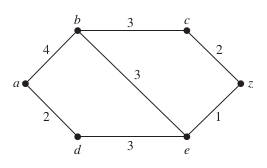
\includegraphics[width=0.4\textwidth]{assets/gr_01.png} 
    \caption{Ví dụ đơn đồ thị với trọng số } % Creates caption underneath graph
    \label{fig:gr_01}
\end{figure}

Tìm đường đi ngắn nhất từ đỉnh $a$ đến đỉnh $z$ trong đồ thị ở hình \ref{fig:gr_01}.\\ 

Trước hết, bắt đầu từ đỉnh $a$, có 2 đỉnh kết nối với $a$ là $b$ và $d$ với trọng số 
lần lượt là $4$ và $2$, đương nhiên $d$ là đỉnh gần $a$ nhất. Chúng ta có thể tìm đỉnh 
gần nhất thứ 2 bằng cách liệt kê tất cả các đường đi với $d$ là đỉnh bắt đầu và đỉnh 
kết thúc không nằm trong tập $\{a, d\}$. Tính từ đỉnh $d$, chỉ có một đường khả dĩ là $e$.
Từ đó ta có tập $\{a, d, e\}$. Tương tự như vậy ta tìm đỉnh tiếp theo với cạnh có trọng số 
nhỏ nhất với $e$ là đỉnh bắt đầu và đỉnh kết thúc không thuộc tập $\{a, d, e\}$, ta được 
đỉnh $z$. Đường đi cuối cùng là $a \to d \to e \to z$. \\

Ví dụ trên thể hiện nguyên lý tổng quát của thuật toán Dijkstra đó là đường đi từ đỉnh $a$
tói đỉnh $z$ có thể được xây dựng bằng cách liệt kê các đường đi và tìm đường có trọng số 
nhỏ nhất để thêm đỉnh đó vào tập đường đi.

Một cách tổng quát ta có thể trình bày thuật toán Dijkstra với lược đồ sau:

\begin{tcolorbox}[colframe=gray,colback=gray!20,left=10pt,right=10pt,top=10pt,bottom=10pt]
    \textbf{Thuật toán Dijkstra} \\
    $G$ là một đơn đồ thị kết nối với trọng số mỗi cạnh dương \\
    $G$ có các đỉnh $a = v_0, v_1, ..., v_n = z$, trọng số 
    $w(v_i, v_j)$ với $w(v_i, v_j) = \infty$ nếu $\{v_i, v_j\}$ không thuộc 
    tập cạnh của $G$

    \begin{itemize}
        \item [] for i = 1 to n 
        \begin{itemize}
            \item [] $L(v_i) = \infty$
        \end{itemize} 
        \item [] $L(a) = 0$
        \item [] $S = \emptyset $ (Khởi tạo các nhãn với nhãn của $a$ là $0$, 
        các nhãn khác bằng $\infty$ và tập $S$ rỗng)
        \item [] while $z \notin S$
        \begin{itemize}
          \item [] $u = a$ đỉnh không thuộc $S$ với $L(u)$ nhỏ nhất
          \item [] $S = S \cup \{u\}$
          \item [] for $v \notin S$
          \begin{itemize}
            \item [] if $L(u) + w(u,v) < L(v)$ then $L(v) = L(u) + w(u,v)$
            (Bước này thêm đỉnh gần nhất vào tập $S$ và cập nhật lại hàm chi phí)
          \end{itemize}
        \end{itemize}
        return $L(z)$ ($L(z)$ là độ dài của đường đi ngắn nhất từ $a$ tới $z$)
    \end{itemize}
  \end{tcolorbox}

\textit{Nhận xét: } Thuật toán Dijkstra đem lại
sự tường minh mà không phải quét qua toàn bộ cấu hình của bài toán, 
ta chỉ cập nhật đỉnh gần với đỉnh cuối cùng nhất, điều đó làm giảm không gian lưu 
trữ so với cách vét cạn (khi ta phải lưu toàn bộ đường đi và chi phí của mọi đường
đi khả dĩ từ đỉnh $a$ tới đỉnh $z$). Độ phức tạp của thuật toán là $O(n^2)$. 
Ta có thể dễ dàng thu được vì ban đầu khi chọn 1 đỉnh, ta cần $(n-1)$ phép so sánh
để tìm được đỉnh gần nhất đầu tiên, tiếp theo ta cần $(n-2)$ phép tính để tìm đỉnh 
gần nhất thứ 2, tiếp tục như vậy cho đến khi thu được đỉnh đích. Số phép tính là tổng 
từ $1$ đến $(n-1)$. \\

Trong thực tế lập trình, chúng ta không nhất thiết phải lưu giá trị cạnh bằng một 
số lớn (vô cùng) mà có thể đánh bằng $0$ và kiểm tra thêm một điều kiện trong vòng 
lặp để tránh sự cồng kềnh của ma trận kề. \\

\href{https://github.com/batman0911/dma_homework/blob/master/hw_02/src/shortest_path.ipynb}{python code} 
    cho bài toán.


\subsection{Bài toán người đưa hàng (TSP)}
Trong mục này chúng ta sẽ xem xét bài toán người đưa hàng đã đề cập ở đầu bài.
Sau khi giải bài toán tìm đường đi ngắn nhất ở mục trước, ta biết rằng bài toán
người đưa hàng không gì khác ngoài việc tìm được đi ngắn nhất khi ta đặt điểm
kết thúc chính là điểm bắt đầu. 
\subsubsection{Thuật toán tìm nghiệm chính xác}
Độ phức tạp thuật toán vét cạn và là $O (n!)$.
Độ phức tạp này tăng rất nhanh theo $n$ . Ví dụ khi bắt đầu từ 1 đỉnh, ta có $(n-1)!$
chu trình Hamilton, tới đỉnh thứ 2 ta còn $(n-2)!$ chu trình Hamilton và tiếp tục như vậy.
Bởi vì ta có thể đi theo thứ tự ngược lại trong chu trình Hamilton nên số chu trình cần
sinh ra để có được lời giải là $(n-1)!/2$. Với số đỉnh bằng $25$, số chu trình được sinh 
ra là $24!/2 \sim 3.1 \times 10^{23}$ - một con số lớn khủng khiếp. Trong thực tế, 
một đơn vị vận chuyển như \textit{Giao hàng tiết kiệm} giao hàng triệu đơn hàng mỗi ngày 
tới các địa điểm khác nhau! Do đó ta gần như không thế tìm được lời giải chính xác của bài 
toán TSP trong thực tế mà cần phải sử dụng các phương pháp xấp xỉ để tìm được một 
đường đi \textit{đủ tốt}.

\subsubsection{Phương pháp xấp xỉ}
Chúng ta sẽ cố gắng đi tìm một cấu hình (chu trình Hamilton) với chi phí không vượt quá
một \textit{ngưỡng} nhất định. Hay nói cách khác $L(H^*_{G}) \leq L(H_{G}) \leq cL(H^*_{G})$,
trong đó $L(H_G)$ là hàm chi phí (tổng các trọng số) của một chu trình Hamilton với
đồ thị $G$ và $H^*_G$ là cấu hình tối ưu của bài toán. Có những thuật toán tìm nghiệm 
xấp xỉ với thời gian đa thức trên đồ thị thỏa mãn bất đẳng thức tam giác với $c = 3/2$. \\

Sử dụng ý tưởng của thuật toán Dijkstra, ta thêm vào tập đỉnh đã đi qua đỉnh lân cận 
gần nhất cho đến khi toàn bộ tập đỉnh đã được đi qua. Độ phức tạp của thuật toán là $O(n^2)$
và ta sẽ cùng xem hệ số $c$ với thuật toán này bằng bao nhiêu. \\

Trước hết, đồ thị $G$ phải thỏa mãn điều kiện bất đẳng thức tam giác 
$w_{ik} + w_{kj} \geq w_{ij}$, với $w_{st}$ là trọng số của cạnh nối đỉnh $s$ và đỉnh $t$.
Điều này cũng khá thực tế khi chi phí bay thẳng từ Hà Nội đến Sài Gòn nên nhỏ hơn là phải 
bay từ Hà Nội vào Đà Nẵng rồi từ Đà Nẵng đi Sài Gòn!

\href{https://github.com/batman0911/dma_homework/blob/master/hw_02/src/travelling_salesman.ipynb}{python code} 
    cho bài toán. \\


% Now we also want to include the graph in our write up.
%  \begin{figure}[H] % places figure environment here   
%     \centering % Centers Graphic
%     \includegraphics[width=0.9\textwidth]{box1.pdf} 
%     \caption{Boxplot of Incumbent Vote share} % Creates caption underneath graph
%   \end{figure}


% Now all we need to answer the question is a neat table. The easiest way to get a nice looking table is to browse to http://www.tablesgenerator.com. Generate your table just like in Word or any other WYSIWYG editor. Then copy and include the code here. I already did that for you.

% \begin{table}[H]
% \centering
% \begin{tabular}{llllllll}
% \multicolumn{1}{c}{\textbf{Variable}} & \multicolumn{1}{c}{\textit{Mean}} & \multicolumn{1}{c}{\textit{Median}} & \textit{Mode} & \textit{Var} & \textit{SD} & \textit{Range} & \textit{IQR} \\ \hline
% Vote                                  & x                                 & x                                   & x             & x            & x           & x              & x            \\
% Growth                                & x                                 & x                                   & x             & x            & x           & x              & x           
% \end{tabular}
% \caption{Measures of central tendency and variability.}
% \label{my-label}
% \end{table}
% You just have to exchange the x for the right value.

\end{document}
